%############################################# ANDRÁS KISS ##########################################
%################################################ 2018 ##############################################
\documentclass[a4paper, 11pt, oneside, bibliography=totoc]{article}
%\def\magyarOptions{hyphenation=huhyphn}
\usepackage{ae,aecompl}
\usepackage[T1]{fontenc}
\usepackage[utf8]{inputenc}
%\usepackage[hungarian]{babel}
\usepackage{indentfirst}
\usepackage{xymtex}
\usepackage{multirow}
\usepackage{gensymb}
\usepackage{upgreek}
\usepackage[geometry]{ifsym}
\usepackage{subfig}
\usepackage[version=3]{mhchem}
\usepackage{float}
\usepackage{textcomp}
\frenchspacing
\usepackage[dvips]{graphicx}
\usepackage{color}
\usepackage{anysize}
\marginsize{3.2cm}{2.8cm}{3cm}{2cm}
\usepackage{enumerate}
\usepackage{cite}
\usepackage{listings}
\usepackage{setspace}
\usepackage{marginnote}
\setstretch{1.2}
\usepackage{xcolor}
\usepackage{listings}

\definecolor{codegreen}{rgb}{0,0.6,0}
\definecolor{codegray}{rgb}{0.5,0.5,0.5}
\definecolor{codepurple}{rgb}{0.58,0,0.82}
\definecolor{backcolour}{rgb}{0.95,0.95,0.92}
\lstdefinestyle{mystyle}{
    backgroundcolor=\color{backcolour},   
    commentstyle=\color{codegreen},
    keywordstyle=\color{magenta},
    numberstyle=\tiny\color{codegray},
    stringstyle=\color{codepurple},
    basicstyle=\footnotesize,
    breakatwhitespace=false,         
    breaklines=true,                 
    captionpos=b,                    
    keepspaces=true,                 
    numbers=left,                    
    numbersep=5pt,                  
    showspaces=false,                
    showstringspaces=false,
    showtabs=false,                  
    tabsize=2
}
\lstset{style=mystyle}


\begin{document}
\title{\emph{DAAD Scholarship} report}
\author{Dr. András Kiss}
\maketitle

In this document I summarize the most important results of my work I have done in the laboratory of prof. Markus Hoth at the Center of Integrative Physiology and Molecular Medicine (CIPMM) in Homburg during the time period of 11th June 2018 -- 10th of August 2018 under the supervision of Dr. Monika Bozem. The work was financially supported by the German Academic Exchange Service (Deutscher Akademischer Austausch Dienst, DAAD).

The main goal of the work was to map the H$_2$O$_2$ production of certain immune cells; natural killer and bystander cells with the Scanning Electrochemical Microscope (SECM). Additionally, new protocols had to be worked out in order to accomplish that goal. Among others, these include:

\begin{itemize}
\item production of 10 $\upmu$m or smaller diameter platinum microelectrodes,
\item calibration and characterization of these,
\end{itemize}

By the time I joined the electrochemistry team at CIPMM, a lot of successful work has already been done \cite{bozem2018electrochemical}. Upon my arrival, Dr. Bozem presented three recently discovered problems which had to be solved before electroactive species like H$_2$O$_2$ and O$_2$ could be mapped in the close vicinity of the immune cells by the SECM:
 
\begin{itemize}
\item high distortion in the images,
\item large amount of noise when the temperature is increased to the physiological 37 $\celsius$,
\item insufficient resolution of the cells due to the relatively large diameter of the platinum microelectrodes.
\end{itemize}

We selected the first one to be worked on. The reason for this is that I have experience with reconstructing SECM images by removing distortion based on theoretical models. The problem is shown in Fig. \ref{fig:deconv}B. When a monocyte is scanned with the SECM, the resulting image is distorted. To investigate the problem, first I have reduced the complexity of the problem by creating a model system. It consisted of an ,,ideal'' step, that has a well defined geometry. The system consisted of a broken glass sheet in a Petri--dish. The broken edge of the glass sheet is very sharp, and creates a good step function. When the Pt UME is scanned above it, the measured current is low when the tip is close to the glass sheet, but once it reaches the edge and it is suddenly in the bulk of the solution, the current increases, because diffusion of the electroactive species (ferrocene) is no longer hindered. This is an ideal setup to study how the image of a near perfect step function is distorted by the scanning process. A sketch of the model system can be seen in Fig. \ref{fig:model1}.

\begin{figure}
\centering
% trim = top left bottom right
% trim = left bottom right top
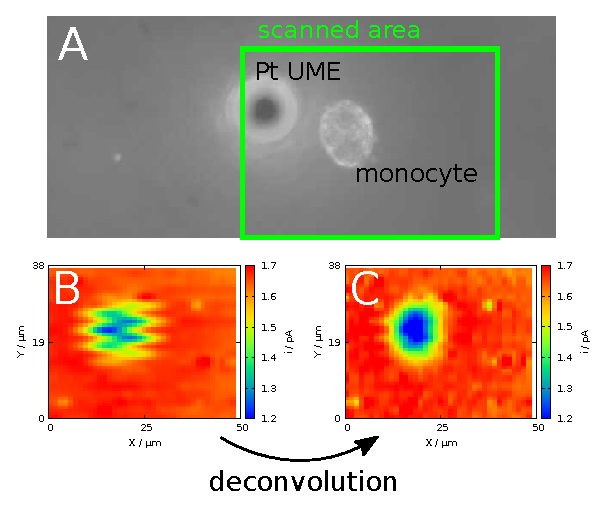
\includegraphics[width=0.8\textwidth]{deconv.eps}
\caption{Figure caption.}
\label{fig:deconv}
\end{figure} 

The result of the SECM scanning is presented in Fig. \ref{fig:step1}. When the system is scanned with a speed of 5 $\upmu$m/s, the image is not distorted. However, when the speed is increased to 10 $\upmu$m/s, the image becomes distorted. This speed is still insufficient to investigate a monocyte with fairly good temporal resolution. Quite surprisingly, after deconvolution, the image besame even more distorted. The explanation is the following. It is a well known fact from hydrodynamics, that when two planes close to each other move relatively to each other in a liquid, and when one reaches the edge of the other, a very strong convective effect is present. This is depicted in Fig. \ref{fig:convective}. This effect increases the current for a short time when the electrode is moving from above the glass sheet cover to the bulk, and the change is more sudden than when it is moving in the opposite direction.

\begin{figure}
\centering
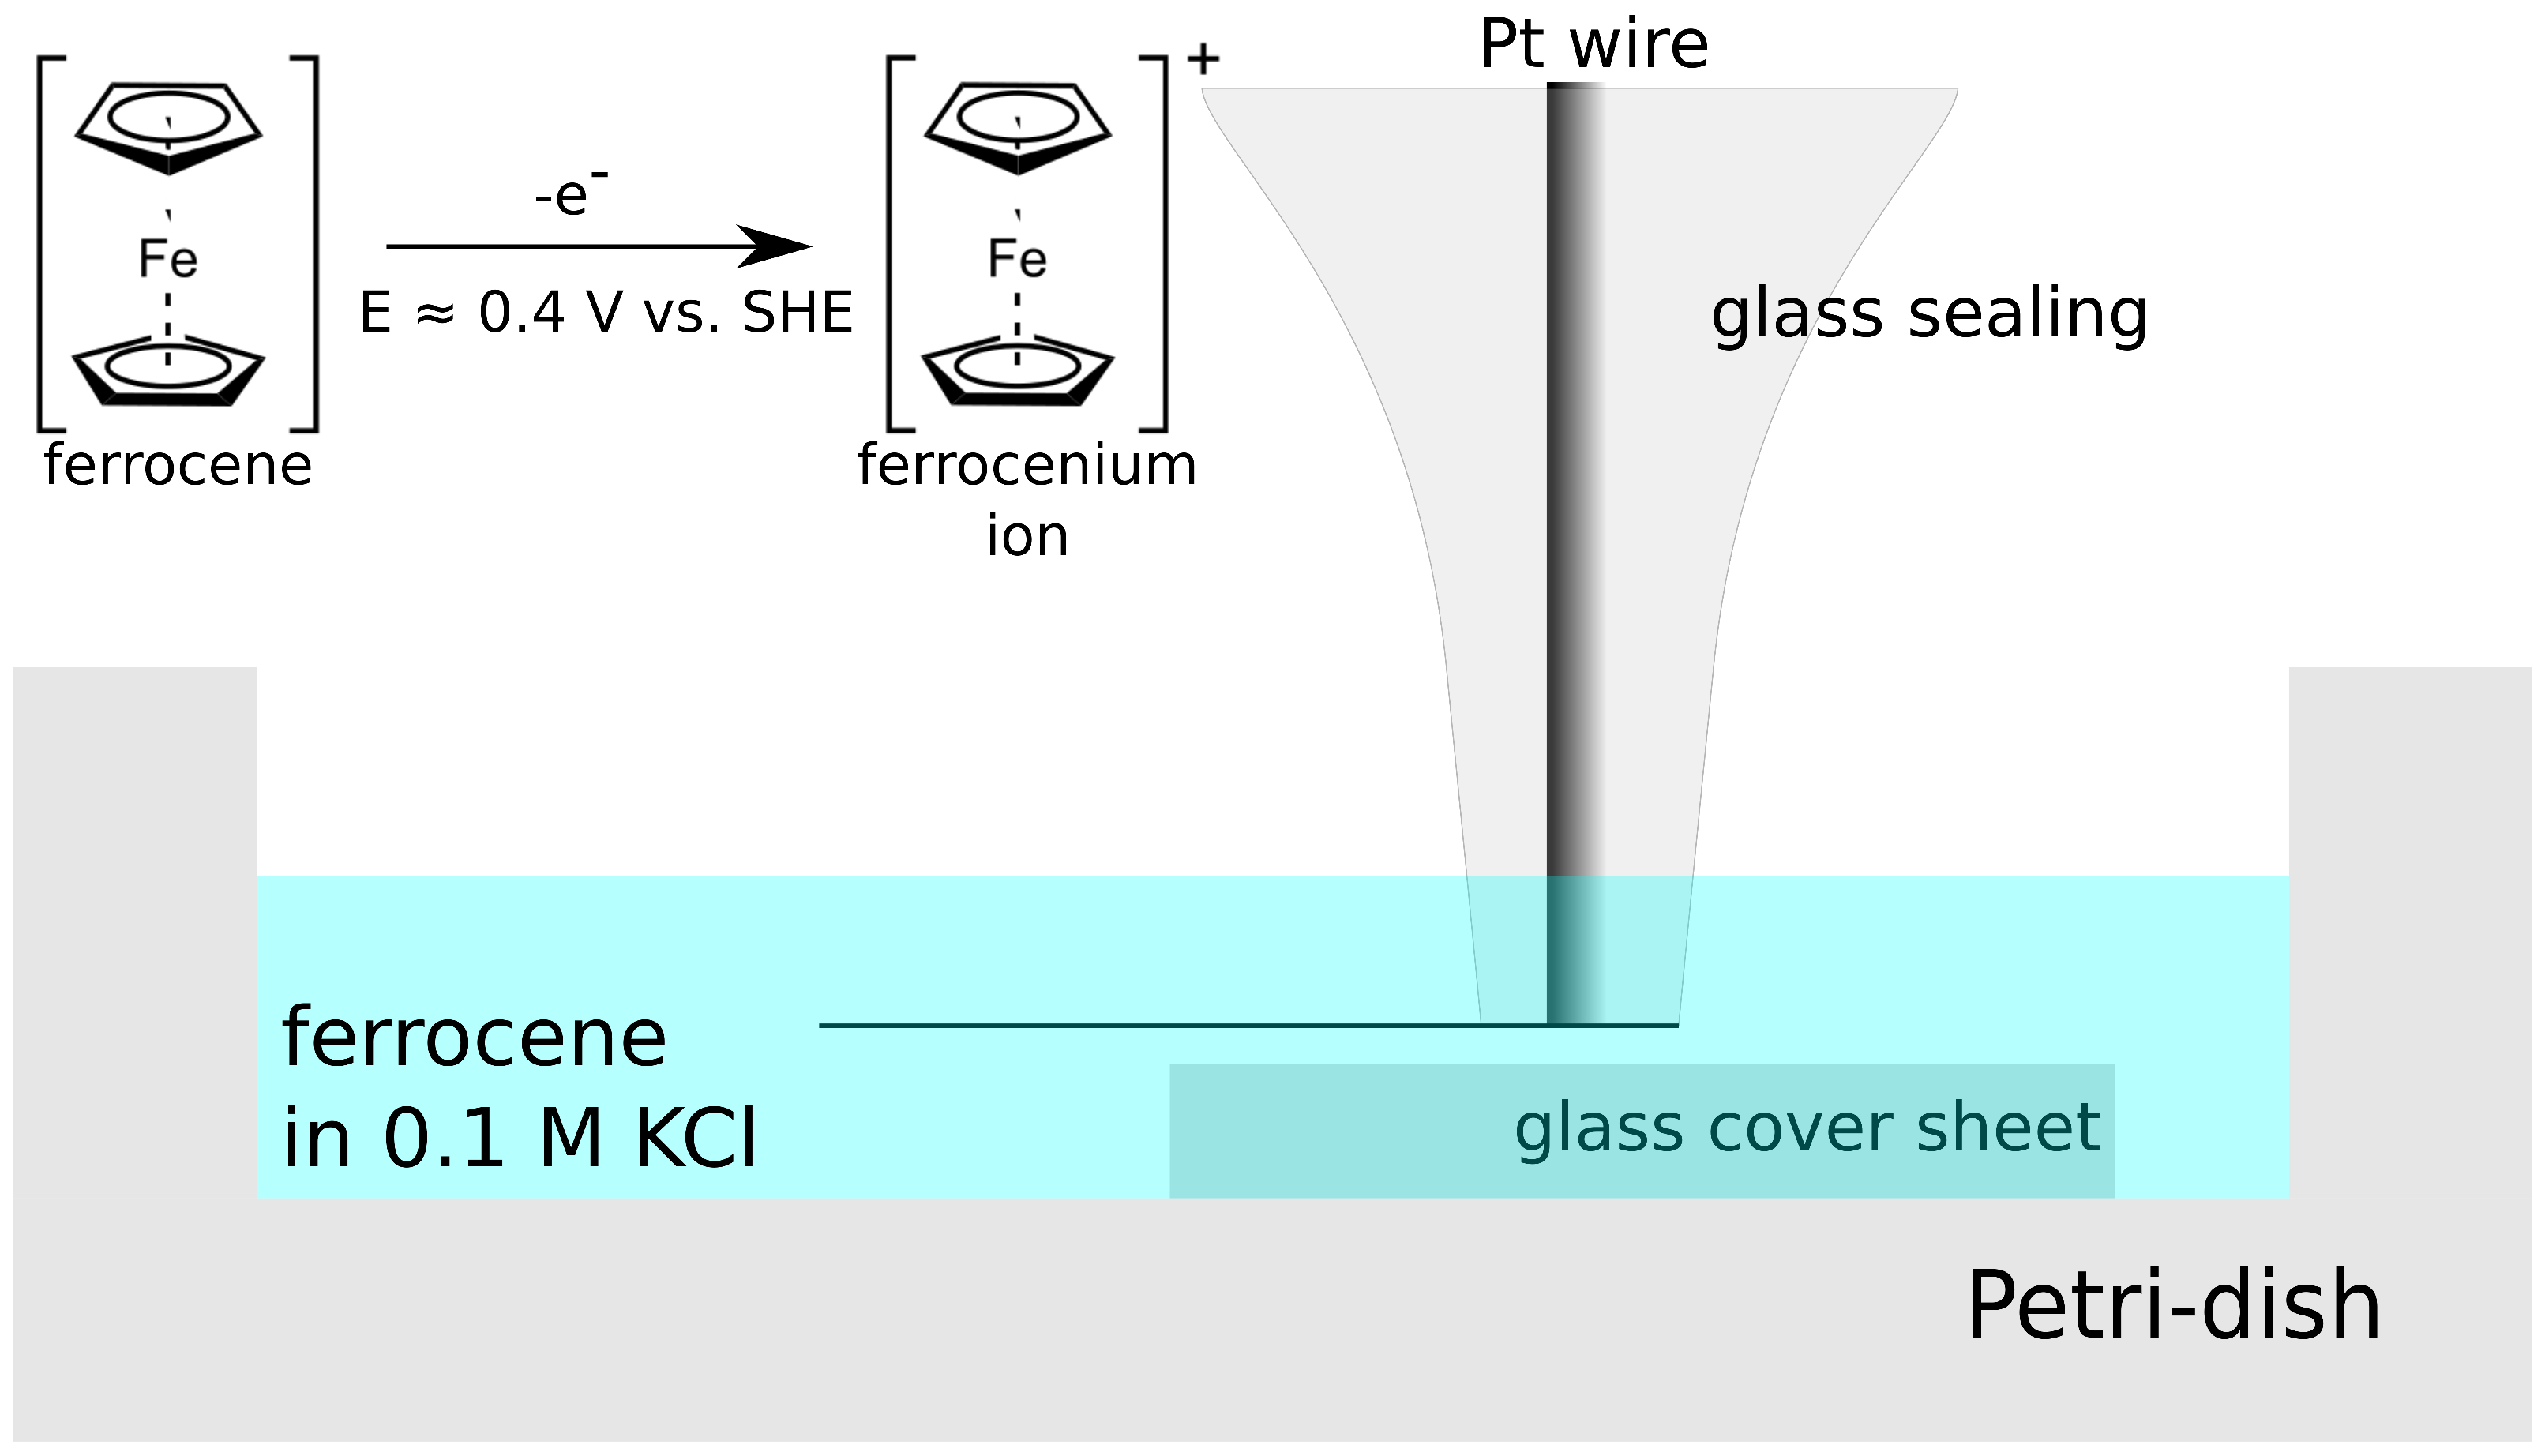
\includegraphics[width=0.7\textwidth]{step.eps}
\caption{Figure caption.}
\label{fig:model1}
\end{figure} 

\begin{figure}
\centering
 \includegraphics[trim = 10mm 60mm 0mm 60mm, clip, width=0.33\textwidth, angle=-90]{1.eps}\includegraphics[trim = 10mm 60mm 0mm 60mm, clip, width=0.33\textwidth, angle=-90]{2_meandered.eps}\includegraphics[trim = 10mm 60mm 0mm 60mm, clip, width=0.33\textwidth, angle=-90]{2_meandered_deconvoluted.eps}

\hspace{1.3cm} 5 $\upmu$m/s \hspace{2.5cm} 10 $\upmu$m/s \hspace{1.2cm} 10 $\upmu$m/s deconvoluted \hfill
\caption{Figure caption.}
\label{fig:step1}
\end{figure}

\begin{figure}
\centering
 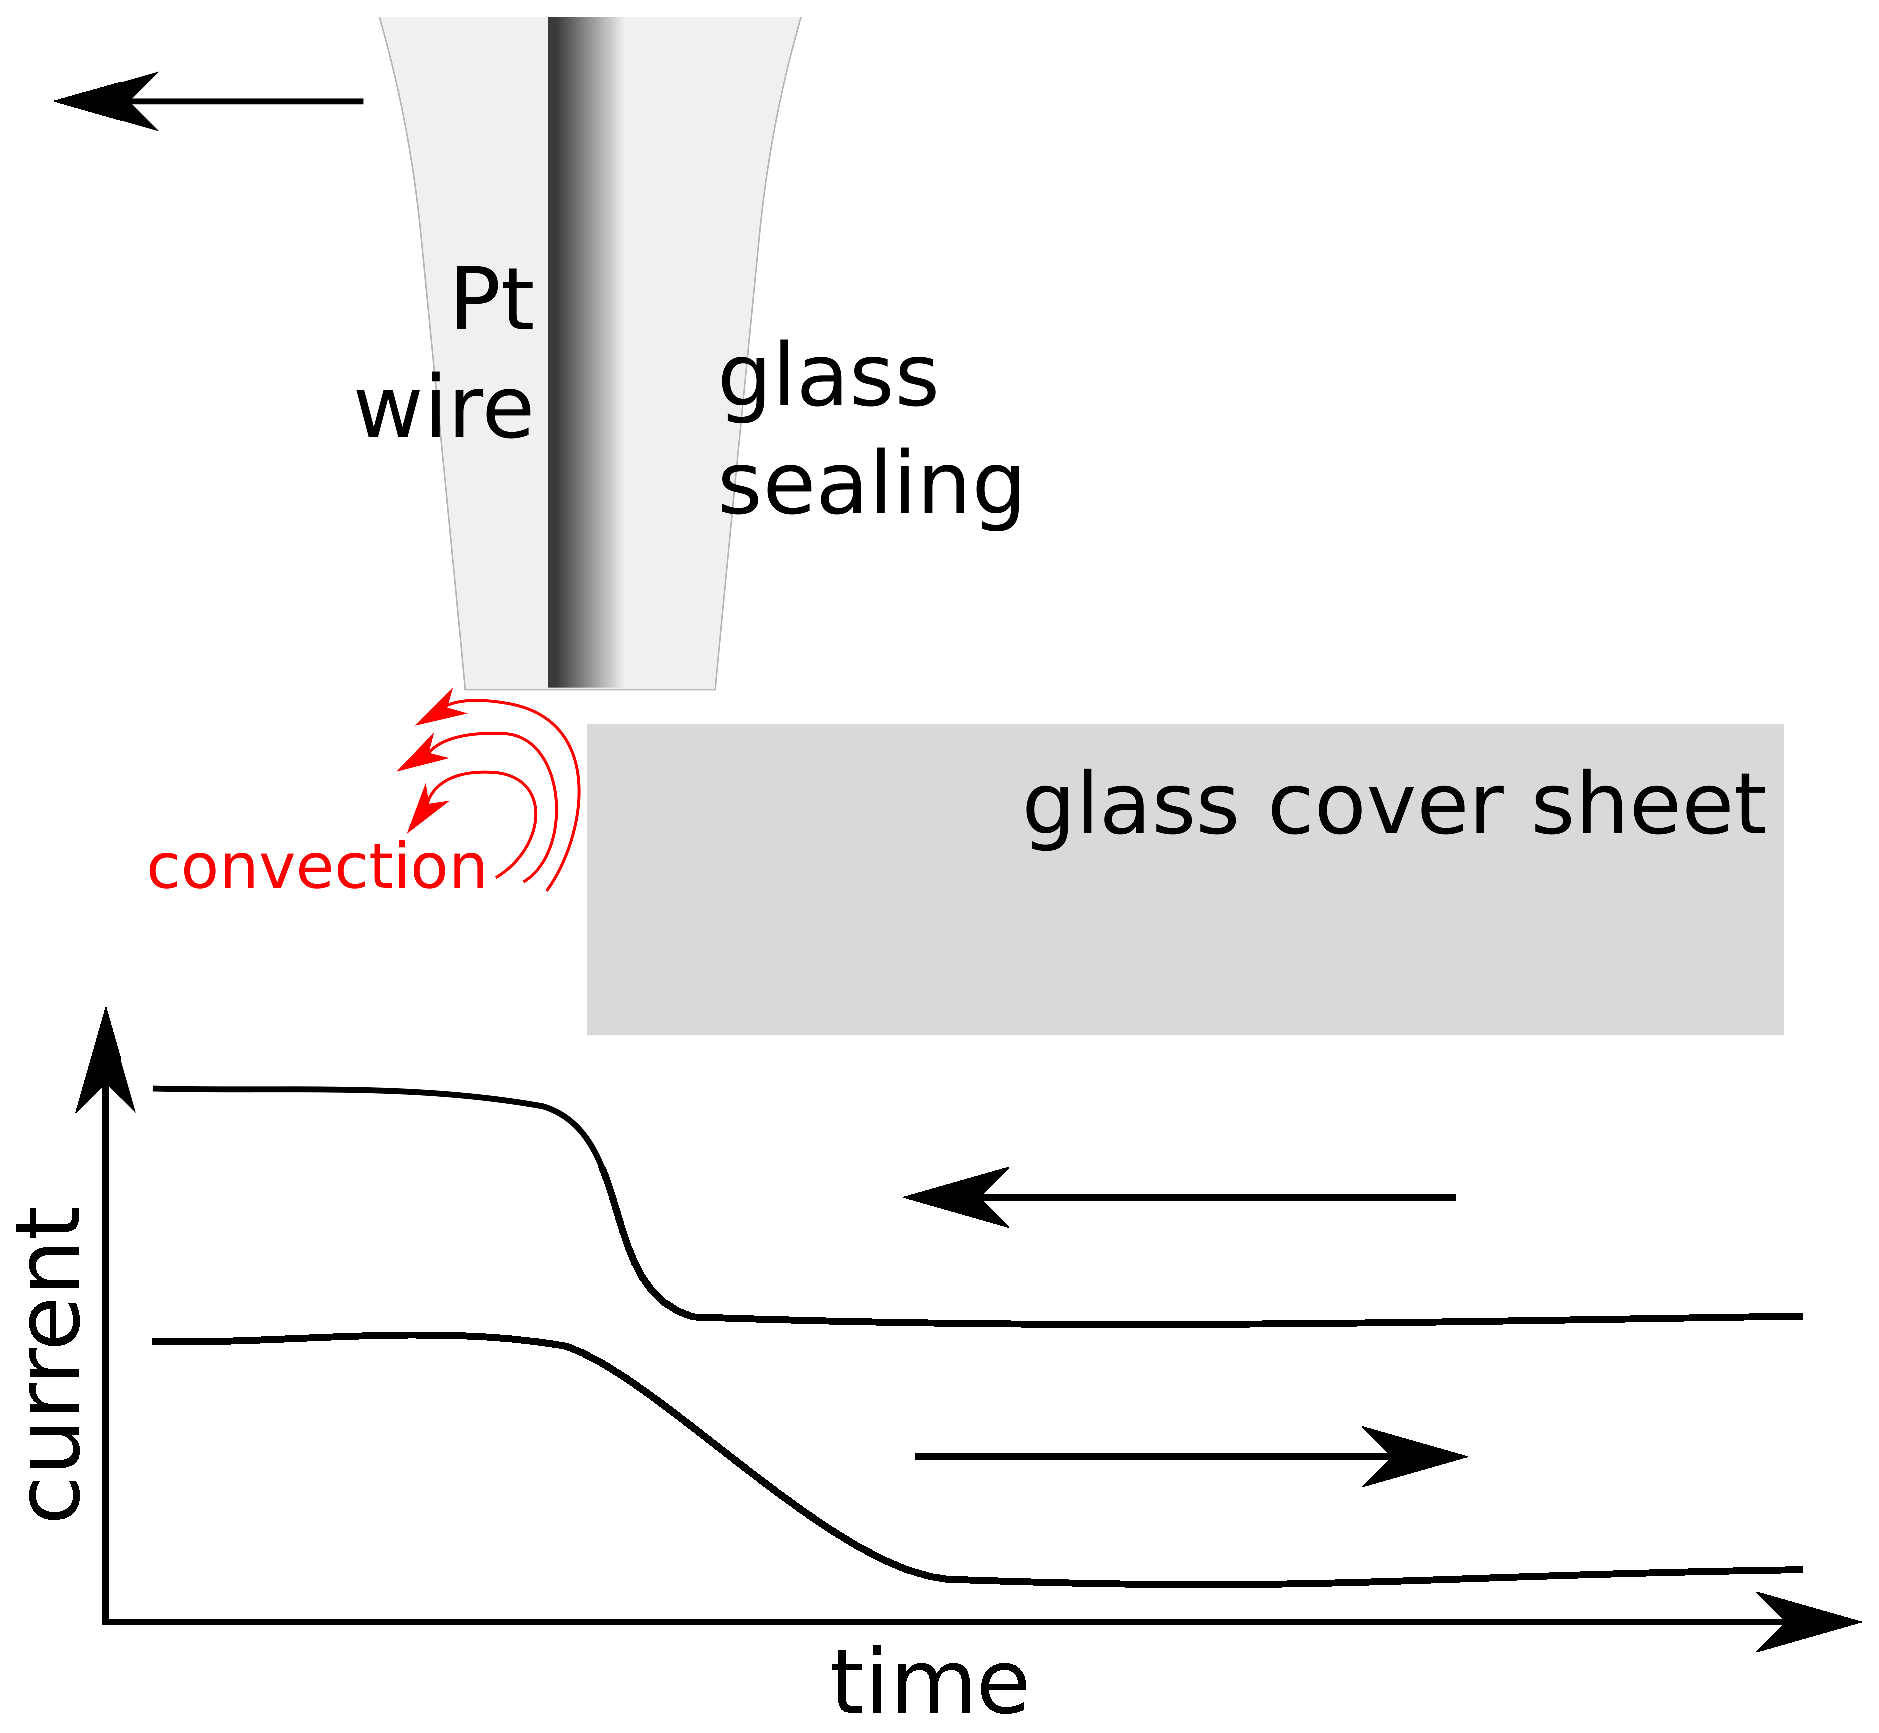
\includegraphics[width=0.6\textwidth]{step_conv.eps}
\caption{Figure caption.}
\label{fig:convective}
\end{figure}

I had to find another model system that acts as a step function. 





The optical microphoto of the scanned monocyte can be seen in Fig. \ref{fig:deconv}A. H$_2$O$_2$ was measured at a d = 10 $\upmu$m Pt microelectrode. The resulting image is distorted (Fig. \ref{fig:deconv}B). This distortion is very similar I have encountered during my PhD studies \cite{kiss2015deconvolution, kiss2015deconvolution2}. In that case, the distortion was caused by the relatively large RC time-constant ot he potentiometric cell. I could solve that by working out a deconvolution algorithm. In this case, the distortion is caused by slow amperometric response that is associated with the Cottrell--equation, but also with the RC time-constant. I have written the following Python program to perform the deconvolution:

\begin{lstlisting}{language=python}
#!/usr/bin/enc python

# Here is a first attempt at porting the deconvolution algorithm
# from FORTRAN to python and applying it on amperometric SECM images.
# The gaussian filter is not yet implemented in the program.
# Right now I do it with the plotting software (gnuplot),
# but it would be better if the python program did it. Also, I haven't
# done the command line argument interpreter yet, so the file name must
# be changed in the code every time. A GUI would be nice, and a live plot
# of the convoluted and deconvoluted image. For that, the XYZ data needs
# to be converted to a matrix.

import numpy as np

conv_img = np.loadtxt("11.txt")
deconv_img = np.copy(conv_img)
e0 = np.float32(conv_img[0][2])
for n in range(0, conv_img.shape[0]):
 deconv_img[n][2] = np.float32((conv_img[n][2]-e0*0.985)/(1-0.985))
 e0 = np.float32(conv_img[n][2])

np.savetxt("11_python_deconvoluted.txt", deconv_img, delimiter=" ")
\end{lstlisting}

After I ran the program above on the dataset plotted in Fig. \ref{fig:deconv}B, the distortion decreased significantly (Fig. \ref{fig:deconv}C). I have managed to successfully deconvolute distorted amperometric SECM images of human immune cells recorded with the HEKA ElProScan SECM at the CIPMM in Homburg.

The SECM image shown in Fig. \ref{fig:deconv}B was measured with an electrode manufactured by Phillip Knapp, PhD student supervised by Dr. Monika Bozem. I have also constructed my own Pt microelectrodes for further experiments. The so-called \emph{RG}--value is a very important parameter of the amperometric microelectrodes. This is the ratio of the diameter of the whole electrode at the tip (insulation + electroactive part) and the electroactive part. I have managed to create Pt UMEs (ultramicro electrodes) with an RG--value of $\approx$ 2.5.

An interesting application of SECM is measuring the O$_2$ concentration in the close vicinity of cells. This can provide information about their metabolic activity. It has great importance in the immune system, where an oxidative burst can significantly influence the O$_2$ concentration nearby the cell. 


Dr. András Kiss

Egyetemi tanársegéd

Általános és Fizikai Kémia Tanszék

Kémiai Intézet

Pécsi Tudományegyetem


2018, június 16

Homburg (Saar)

Németország


\bibliography{report}{}
\bibliographystyle{plain}


\end{document}
